%++++++++++++++++++++++++++++++++++++++++
% Don't modify this section unless you know what you're doing!
\documentclass[letterpaper,12pt]{article}
\usepackage{tabularx} % extra features for tabular environment
\usepackage{amsmath}  % improve math presentation
\usepackage{graphicx} % takes care of graphic including machinery
\usepackage[margin=1in,letterpaper]{geometry} % decreases margins
\usepackage{cite} % takes care of citations
\usepackage[final]{hyperref} % adds hyper links inside the generated pdf file
\usepackage{pgfplotstable, booktabs}
\usepackage{placeins}
\usepackage{tabularray}
\usepackage{titlesec}
\usepackage{fancyhdr}
\usepackage{empheq}
\usepackage{amssymb}
\usepackage{sectsty}
\usepackage{tcolorbox}
\usepackage{listings}
\usepackage{xcolor}
\usepackage{parskip}
\usepackage{cancel}
\usepackage{enumitem}
\usepackage{amsmath}
\usepackage{mathrsfs}
\usepackage{physics}
\usepackage{subcaption}


\definecolor{codegreen}{rgb}{0,0.6,0}
\definecolor{codegray}{rgb}{0.5,0.5,0.5}
\definecolor{codepurple}{rgb}{0.58,0,0.82}

\lstdefinestyle{mystyle}{
    commentstyle=\color{codegreen},
    keywordstyle=\color{codepurple},
    numberstyle=\tiny\color{codegray},
    stringstyle=\color{codegreen},
    basicstyle=\ttfamily\small,
    breakatwhitespace=false,         
    breaklines=true,                 
    captionpos=b,                    
    keepspaces=true,                                                     
    showspaces=false,                
    showstringspaces=false,
    showtabs=false,                  
    tabsize=4
}

\lstset{style=mystyle}
  
\newcommand*\widefbox[1]{\fbox{\hspace{0em}#1\hspace{0em}}}

\pagestyle{fancy}
\fancyhf{} % Clear all header and footer fields
\fancyhead[L]{MEC E 420}
%\fancyhead[C]{Center Header}
\fancyhead[C]{Lab 1}
\fancyhead[R]{Alex Diep}

\fancyfoot[C]{\thepage}

\pgfplotsset{compat=1.18} 
\titleformat*{\section}{\Large\bfseries}
\titleformat*{\subsection}{\large\bfseries}



\renewcommand{\thesection}{Question \arabic{section}}
\renewcommand{\thesubsection}{(\alph{subsection})}
\renewcommand*{\arraystretch}{1.5}

\hypersetup{
	colorlinks=true,       % false: boxed links; true: colored links
	linkcolor=blue,        % color of internal links
	citecolor=blue,        % color of links to bibliography
	filecolor=magenta,     % color of file links
	urlcolor=blue         
}

%++++++++++++++++++++++++++++++++++++++++
\begin{document}

% Consider laminar flow between two parallel plates (Fig. 1). Plates extend infinitely in x and
% z directions. The following assumptions are made:
% • the flow is at steady state (no time dependency)
% • the fluid is incompressible, ideal and Newtonian
% • the temperature of the bottom plate is Tb and the upper plate is at temperature Tu
% • vy = vz = 0
% • vx = vx(y), T = T(y)
% Figure 1: Problem statement: fluid flow between two parallel plates. The bottom plate is
% fixed, the upper plate is moving horizontally with velocity uw. The fluid is incompressible
% and Newtonian.


\section{}
\textit{Write down the full set of governing equations (continuity, momentum and energy).}

\begin{figure}[h]
    \centering
    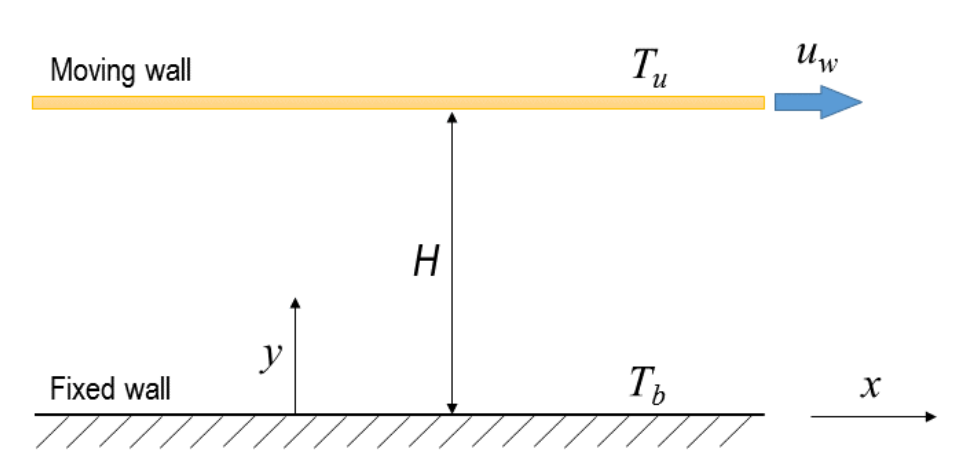
\includegraphics[width=0.5\textwidth]{Questions/Figures/Q1 diagram.png}
    \caption{Fluid flow betweeen parallel plates. The bottom plate is fixed, the upper plate is moving horizontally with velocity $u_w$. THe fluid is incompressible and Newtonian.}
    \label{fig:Q1 diagram}
\end{figure}

\subsection*{Solution}
We first begin with continuity, 
\begin{align*}
    \Aboxed{\frac{\partial \rho}{\partial t} + \vec{u} \cdot \nabla \rho + \rho (\nabla \cdot \vec{u}) &= 0}
\end{align*}
then, the momentum equation,
\begin{align*}
    \Aboxed{\frac{\partial}{\partial t} (\rho u_i) + \frac{\partial}{\partial x_j} (\rho u_i u_j) &= -\frac{\partial P}{\partial x_i} + \frac{\partial}{\partial x_j} \left[ \mu \left( \frac{\partial u_i}{\partial x_j} + \frac{\partial u_j}{\partial x_i} \right) \right] - \frac{\partial}{\partial x_i} \left(\frac{2}{3} \mu \frac{\partial u_k}{\partial x_k} \right) + \rho b_i}
\end{align*}
lastly, the energy equation,
\begin{align*}
    \Aboxed{\rho C_p \left(\frac{\partial T}{\partial t} + \vec{v} \cdot \nabla T \right) &= k \nabla^2 T + \frac{\mu}{2} \Phi^2}
\end{align*}
where $\Phi_{i, j} = \left( \frac{\partial u_i}{\partial x_j} + \frac{\partial u_j}{\partial x_i} \right)$.



\section{}
\textit{Provide a clean vector plot of the flow velocity that clearly illustrates the mixing of two
streams of air. Particularly, what do these vector results indicate about the flow physics?
Use screenshots and other illustrations to support your statement.}

\subsection*{Solution}
\begin{figure}[h]
    \centering
    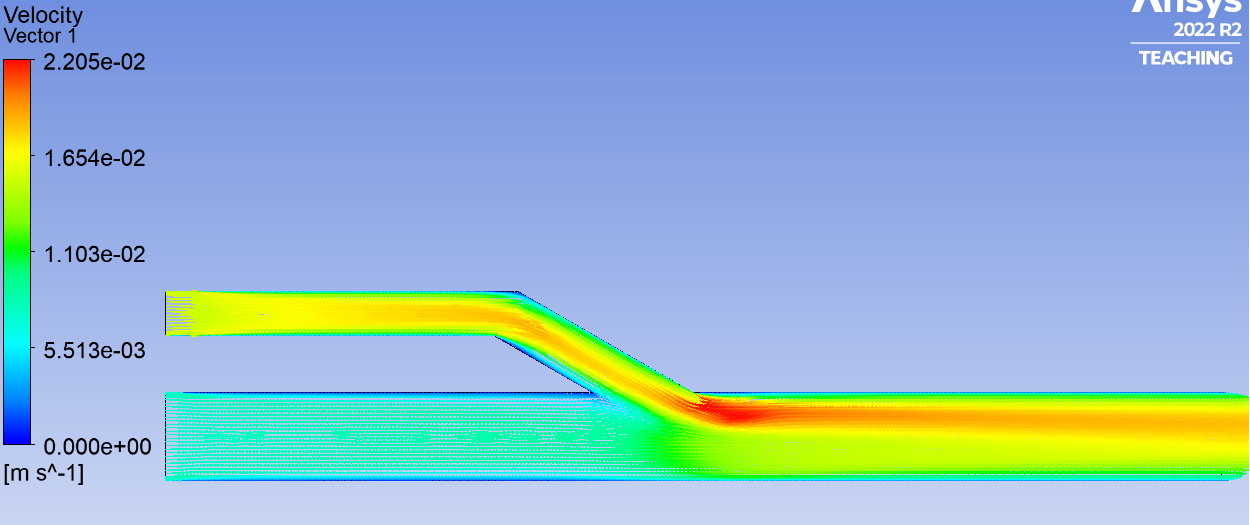
\includegraphics[width=0.8\textwidth]{Questions/Figures/velocity vector.png}
    \caption{Vector field plot of the flow velocity}
    \label{fig:contour}
\end{figure}

The velocity plot shows much of the same information as the contour plot. The plot clearly illustrates the mixing of two streams of air. The plot indicates that the higher velocity flow `pushes' down the lower velocity field. As the flow continues, the stream seems to `mix' the velocities to an average velocity as it approaches the outlet.

For both the upper and lower flows, a boundary layer can be seen developing starting from the inlet. The boundary layer is more pronounced for the upper flow.

Also, the velocity of the upper stream increases around the corner where the flows mix.
\section{}
\textit{Solve the simplified momentum equation.}

\subsection*{Solution}
Using no-slip boundary conditions, the boundary conditions are 
\begin{align*}
    u_x(0) &= 0 \\
    u_x(H) &= u_w
\end{align*}

The simplified momentum equation in the $x$-direction is given by
\begin{align*}
    \frac{\partial^2 u_x}{\partial y^2} &= 0
\end{align*}
which has the general solution
\begin{align*}
    u_x(y) &= A y + B
\end{align*}
where $A$ and $B$ are constants. Applying the boundary conditions, we find
\begin{align*}
    u_x(0) &= B = 0 \\
    u_x(H) &= A H = u_w
\end{align*}
which gives
\begin{align*}
    u_x(y) &= \frac{u_w}{H} y
\end{align*}
This linear profile is also known as Couette flow. Next, the simplified momentum equation in the $y$-direction is given by
\begin{align*}
    \frac{\partial P}{\partial y} &= 0
\end{align*}
which has the general solution
\begin{align*}
    P &= C(z)
\end{align*}
where $C(z)$ is a function of $z$. Lastly, the simplified momentum equation in the $z$-direction is given by
\begin{align*}
    \frac{\partial P}{\partial z} &= -\rho g
\end{align*}
which has the general solution
\begin{align*}
    P(z) &= -\rho g z + D
\end{align*}
where $D$ is a constant.

So in summary, 
\begin{empheq}[box=\fbox]{align*}
    \vec{u} &= \left[\frac{u_w}{H} y\right] \hat{i} \\
    P &= -\rho g z + D
\end{empheq}
\section{}
% \textit{Substitute approximations obtained in Questions 2 and 3 back
% into equation derived in Question 1. Rearrange the obtained equation into a form}
\textit{Substitute approximations obtained in Questions 2 and 3 back into equation derived in Question 1. Rearrange the obtained equation into a form that can be used to solve for $\hat{T}_P$.}
\begin{align*}
    a_P T_P &= a_W T_W + a_E T_E 
\end{align*}
\textit{and identify coefficients $a_P$, $a_W$, $a_E$, $q_{T}^{u}$, and $q_{T}^{P}$.} \\

Substituting back into the equation derived in Question 1,
\begin{align*}
    \hat{T}_P - \hat{T}_W &= \frac{1}{\text{Pe}} \left(\frac{\hat{T}_E - 2\hat{T}_P + \hat{T}_W}{\Delta x}\right) 
\end{align*}
Rearranging,
\begin{align*}
    %\left[\frac{2}{\text{Pe}\Delta x} + 1\right]\hat{T}_P &= \left[\frac{1}{\text{Pe}\Delta x} + 1\right]\hat{T}_W + \left[\frac{1}{\text{Pe}\Delta x}\right]\hat{T}_E + [0] q_{T}^{u} 
    \underbrace{\left[\frac{2}{\text{Pe}\Delta x} + 1\right]}_{a_P}\hat{T}_P &= \underbrace{\left[\frac{1}{\text{Pe}\Delta x} + 1\right]}_{a_W}\hat{T}_W + \underbrace{\left[\frac{1}{\text{Pe}\Delta x}\right]}_{a_E}\hat{T}_E + [0] q_{T}^{u} + [0] q_{T}^{P}
\end{align*}

\end{document}